\documentclass[tikz,border=2]{standalone}

\def\hh{0000}
%\def\hh{.00009}
\pgfmathsetmacro{\hhh}{0.8*\hh}
\pgfmathsetmacro{\hout}{min(0.3, \hh)}

\def\aa{1}

\pgfmathsetmacro{\aminy}{\aa-\hh}

\pgfmathsetmacro{\bb}{1.2*\aa}
\pgfmathsetmacro{\windowstart}{0.3*\aa}
\pgfmathsetmacro{\windowend}{0.6*\aa}
\pgfmathsetmacro{\weights}{0.02*\aa}
\pgfmathsetmacro{\rollerboxheight}{0.1*\aa}
\pgfmathsetmacro{\rollerboxwidth}{1.1*\bb}
\pgfmathsetmacro{\framewidth}{.05*\bb}




\begin{document}
  \begin{tikzpicture}[scale=8]
    %\fill[black] (0, 0)  rectangle (\bb, \aa);
    \clip (0,0) rectangle (\bb+\framewidth, \aa+\rollerboxheight);
    \node[] at (0.52*\bb,0.5*\aa)  {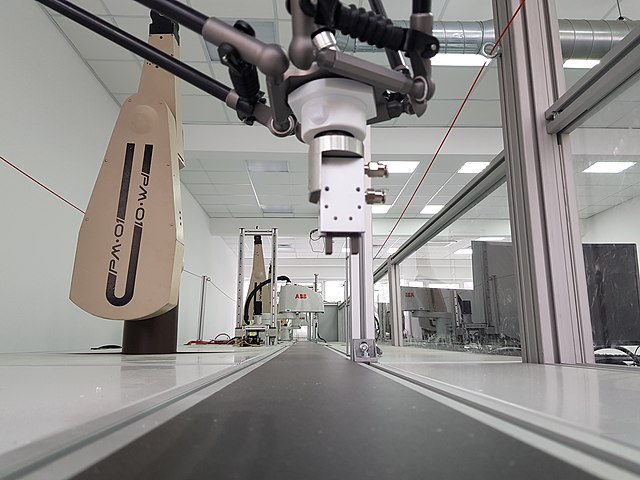
\includegraphics[width=11 cm]{manufacture.jpg}};
    %\shade[ball color=black!10] (0,0) -- (\framewidth,0) -- (\framewidth, \aa)
    %-- (0, \aa) -- cycle;
    %The frame
    \shade[bottom color=black!60, top color=black!10] (0,0) -- (\framewidth,0) -- (\framewidth, \aa)
    -- (0, \aa) -- cycle;
    \begin{scope}[xshift=\bb cm]
      \shade[bottom color=black!60, top color=black!10] (0,0) -- (\framewidth,0) -- (\framewidth, \aa)
      -- (0, \aa) -- cycle;
    \end{scope}
    
    % The roller box
    \begin{scope}[yshift=\aa cm]
      \shade[bottom color=black!80, top color=black!10] (0,-0.001*\aa) -- (\bb+\framewidth,-0.001*\aa)
      -- (\bb+\framewidth, \rollerboxheight)-- (0, \rollerboxheight) -- cycle;
    \end{scope}

    % The curtain
    \begin{scope}[yshift=\hh cm]
      \clip (0,0) rectangle (\bb, \aminy);
      % Bottom part of curtain
      \shade[top color=blue!70, bottom color=blue!70!black] (\framewidth,0) rectangle (\bb, \windowstart);
      % Top part of curtain
      \shade[top color=blue!70, bottom color=blue!70!black] (\framewidth,\windowend) rectangle (\bb, \aa);
      % The weights at bottom of curtain
      \shade[bottom color=black!60, top color=black!10] (\framewidth,\weights) -- (\bb+\framewidth,\weights)
      -- (\bb+\framewidth, \weights+\weights)-- (\framewidth, 2*\weights) -- cycle;
      % The window
      \fill[color=white, opacity=0.4] (\framewidth,\windowstart) -- (\bb+\framewidth,\windowstart)
      -- (\bb+\framewidth, \windowend)-- (\framewidth, \windowend) -- cycle;
      
    \end{scope}    
\end{tikzpicture}%
\end{document}